
\section{Experiments: Planar Projections}
The selected planar projections for the experimentation are mentioned below:
\begin{itemize}
    \item Azimuthal Equidistant
    \item Wagner VII
    \item Lambert Azimuthal Equal Area
    \item Airy
\end{itemize}

% \subsection{Lambert Azimuthal Equal Area}
\begin{figure}[H]
    \centering
    \begin{minipage}{0.30\textwidth}
        \centering
        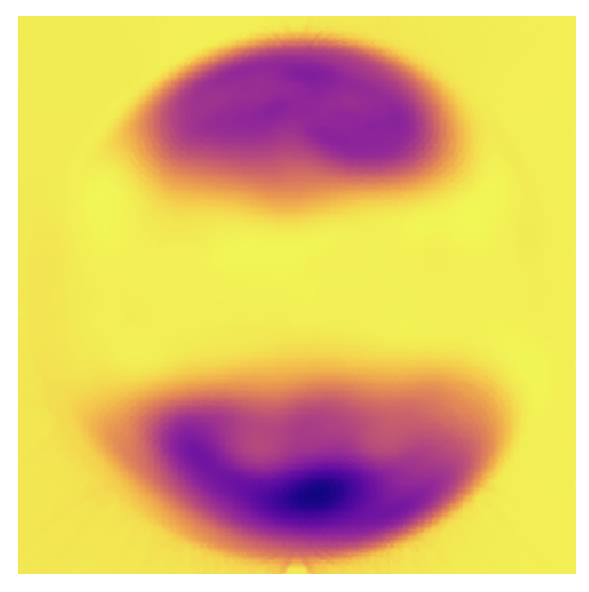
\includegraphics[width=0.9\linewidth]{figures/chapter-8/geopoth_laea.png}
        \caption{ Geopotential height raster data as Lambert Azimuthal Equal Area projected}
        \label{fig:laea_geopoth_raster}
    \end{minipage}\hfill
    \begin{minipage}{0.30\textwidth}
        \centering
        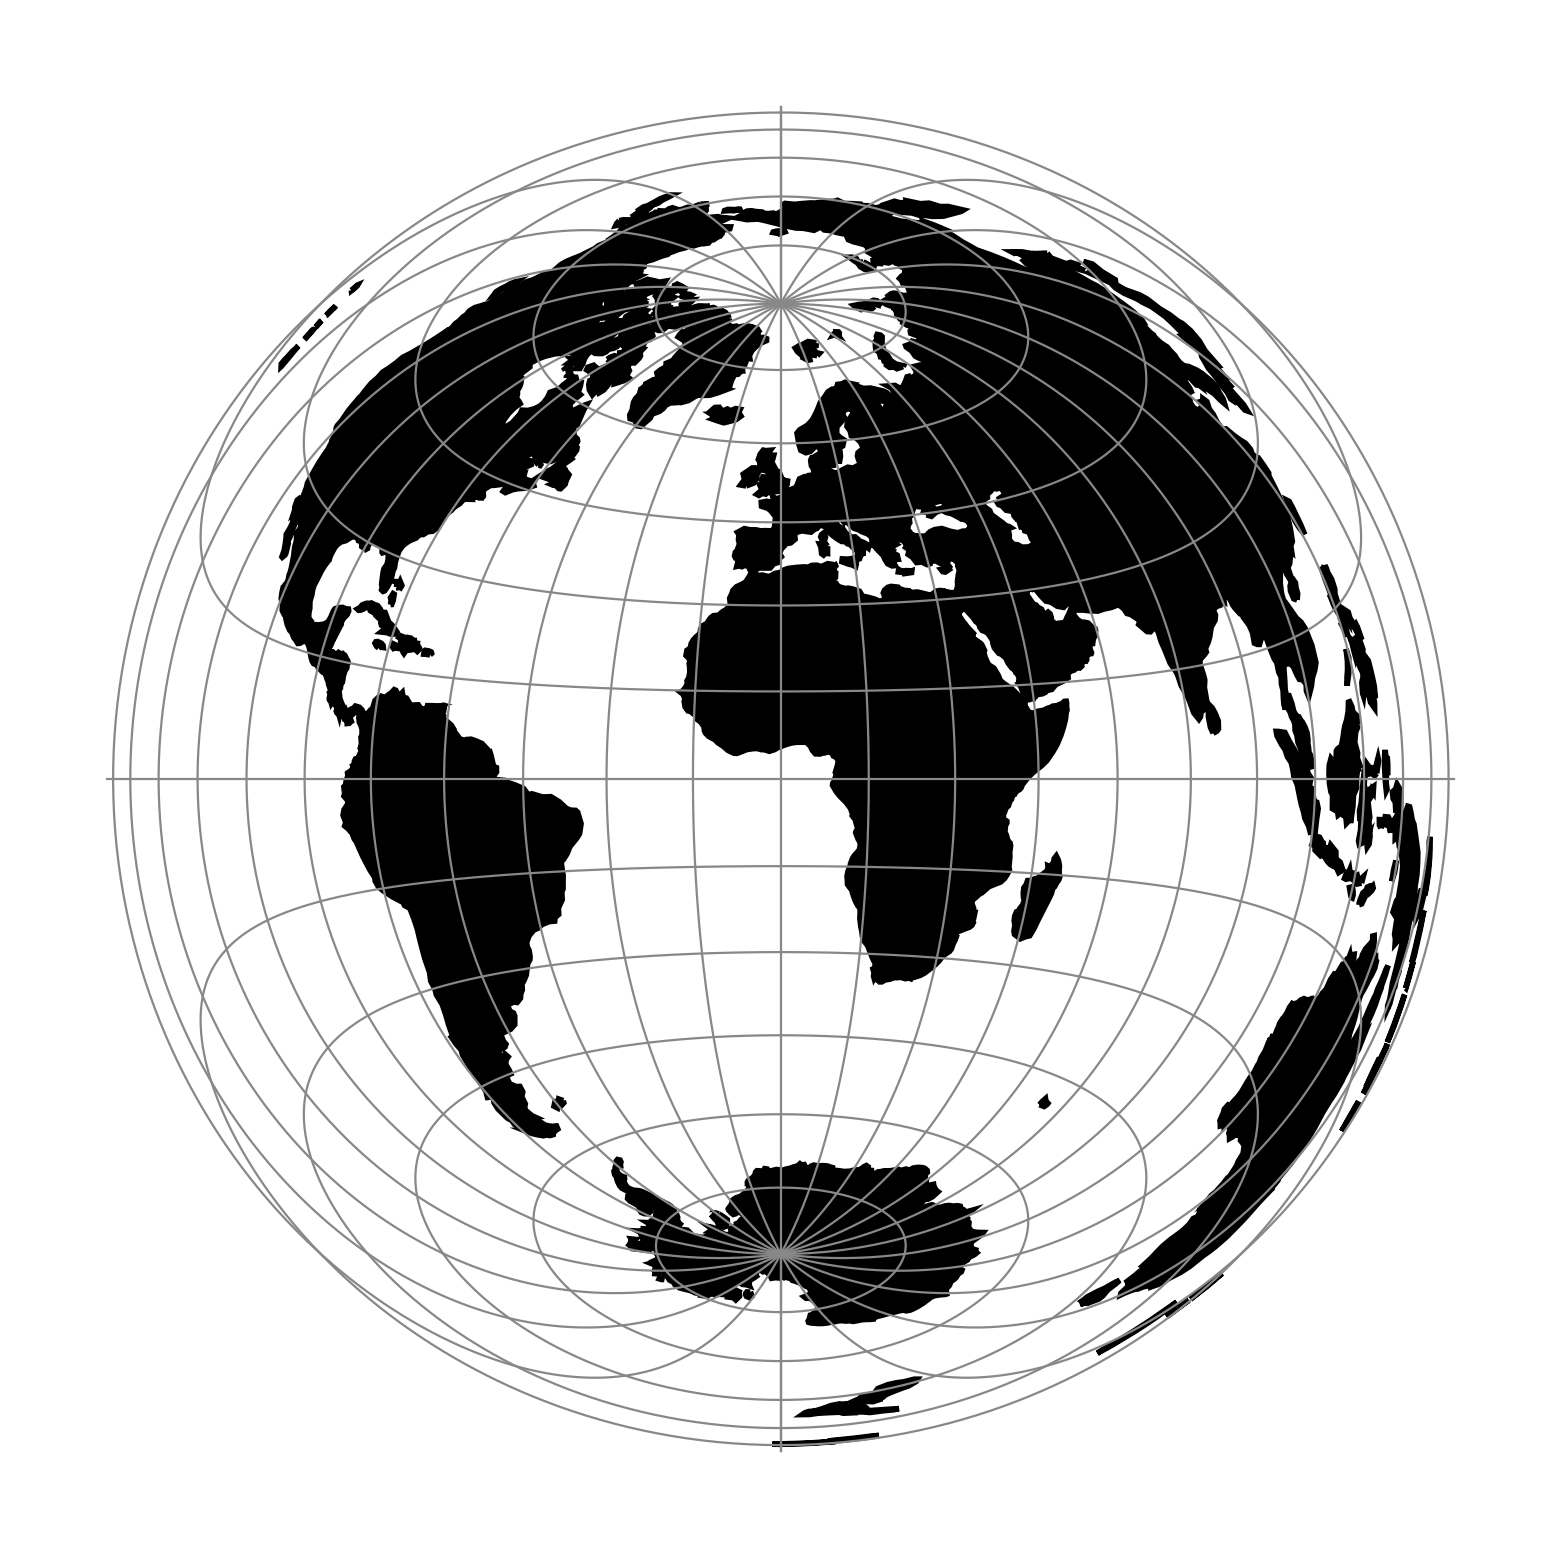
\includegraphics[width=0.9\linewidth]{figures/chapter-8/laea.png}
        \caption{Lambert Azimuthal Equal Area (Source \cite{PROJ_SITE})}
        \label{fig:laea_proj}
    \end{minipage}\hfill
    \begin{minipage}{0.30\textwidth}
        \centering
        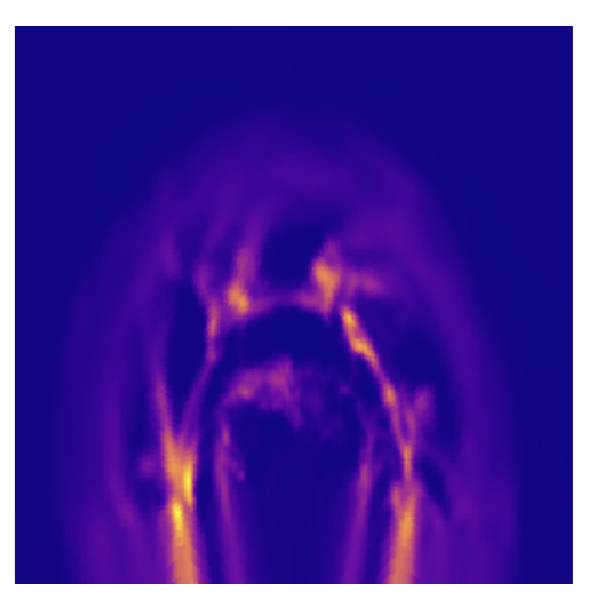
\includegraphics[width=0.9\linewidth]{figures/chapter-8/prect_lcca.png}
        \caption{Precipitation raster data as Lambert Azimuthal Equal Area projected}
        \label{fig:laea_prect_raster}
    \end{minipage}\hfill
\end{figure}

% \subsection{Wagner VII}
% \begin{figure}[H]
%     \centering
%     \begin{minipage}{0.30\textwidth}
%         \centering
%         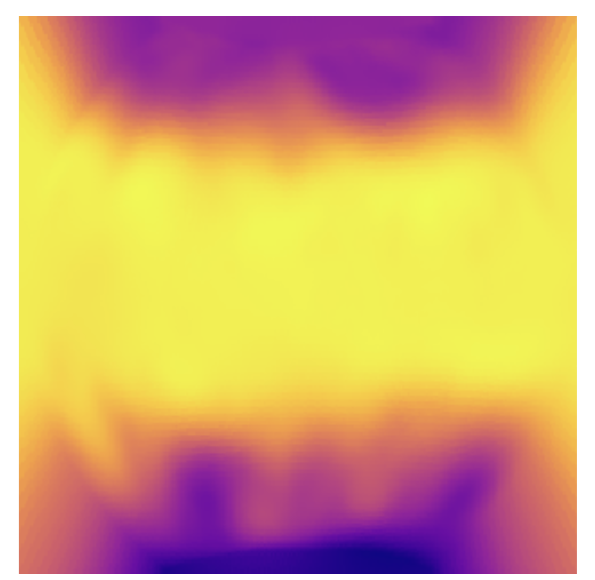
\includegraphics[width=0.9\linewidth]{figures/chapter-8/geopoth_wag.png}
%         \caption{ Geopotential height raster data as Wagner VII projected}
%         \label{fig:wag_geopoth_raster}
%     \end{minipage}\hfill
%     \begin{minipage}{0.30\textwidth}
%         \centering
%         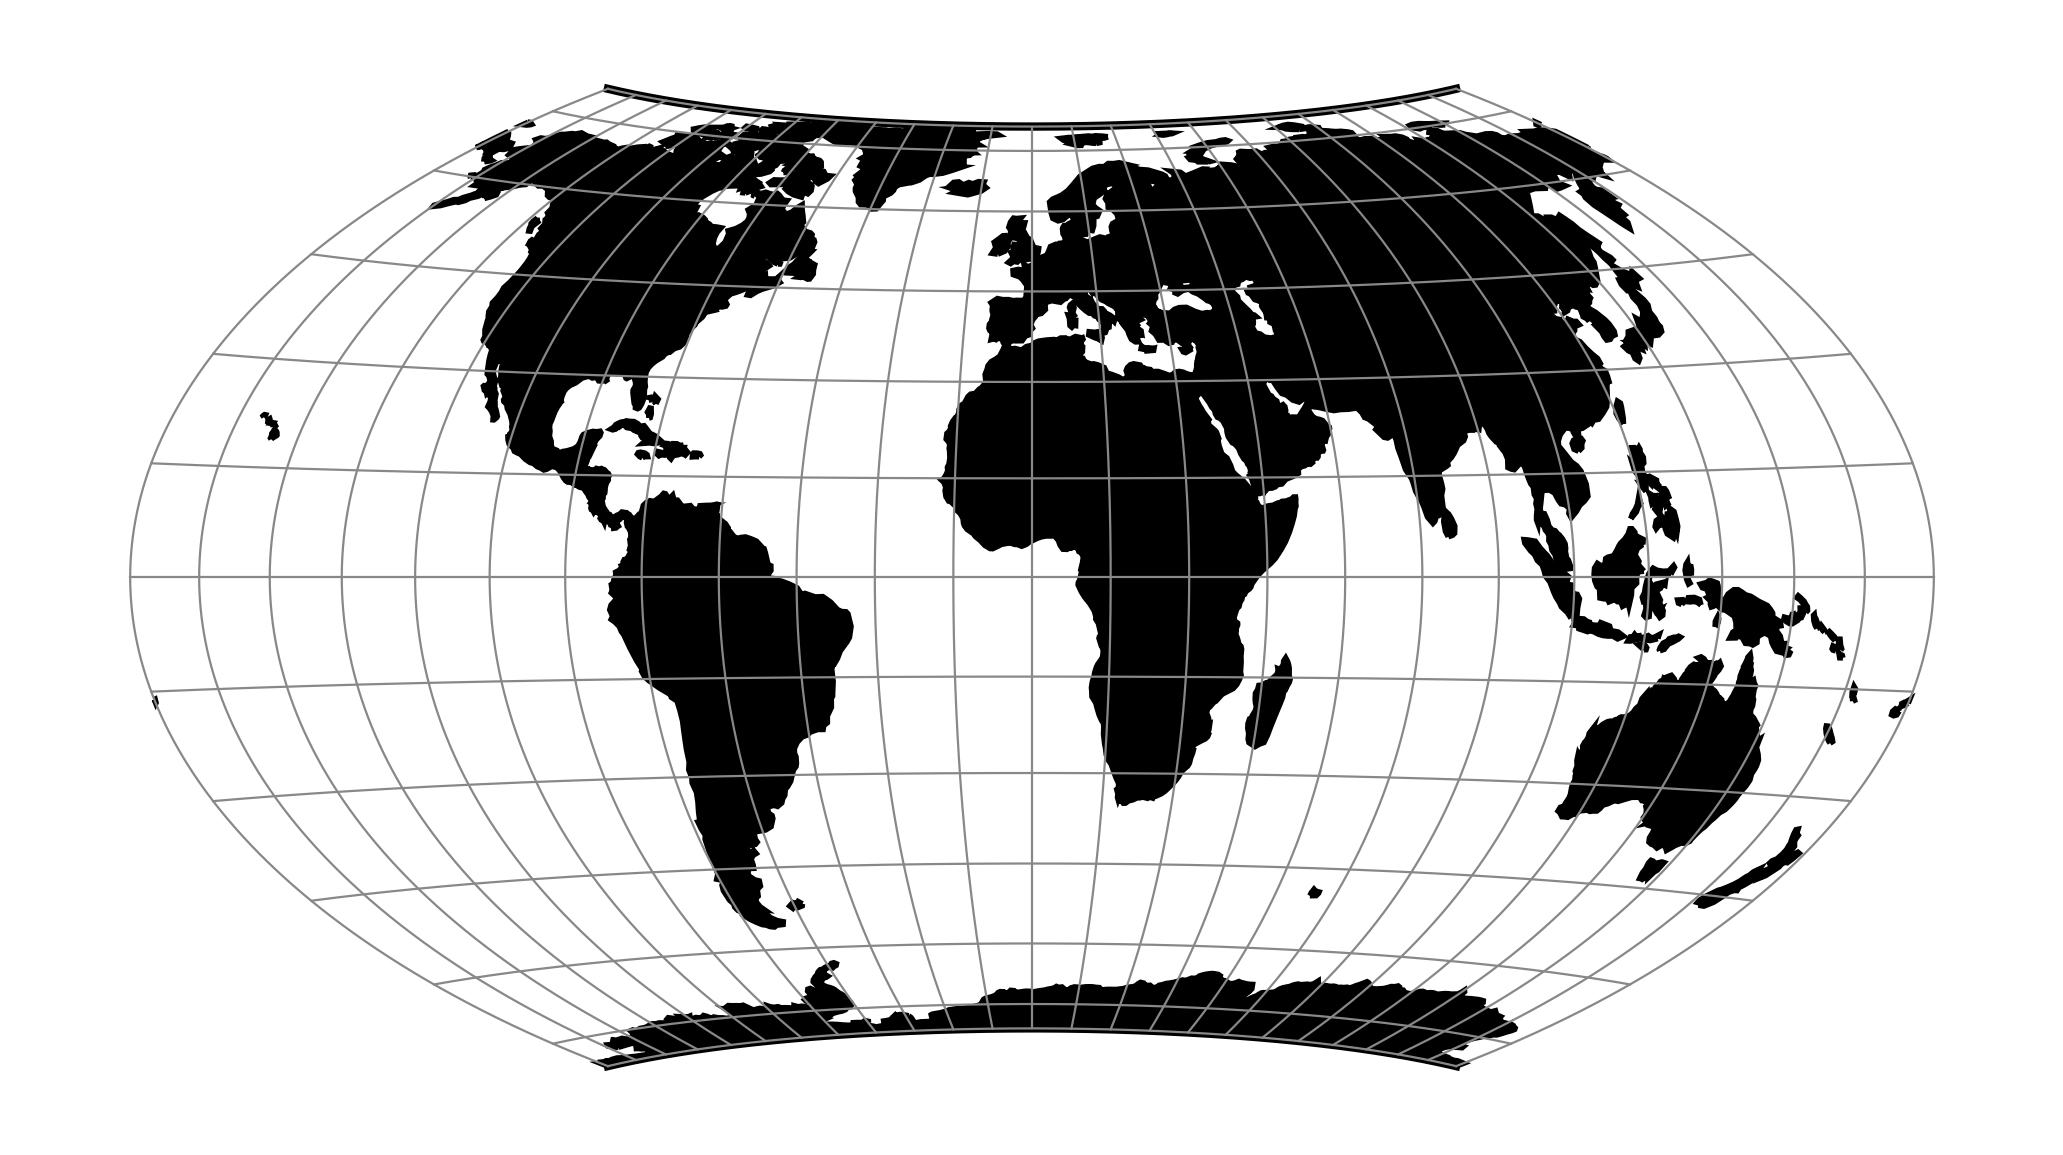
\includegraphics[width=0.9\linewidth]{figures/chapter-8/wag7.png}
%         \caption{Wagner VII (Source \cite{PROJ_SITE})}
%         \label{fig:wag_proj}
%     \end{minipage}\hfill
%     \begin{minipage}{0.30\textwidth}
%         \centering
%         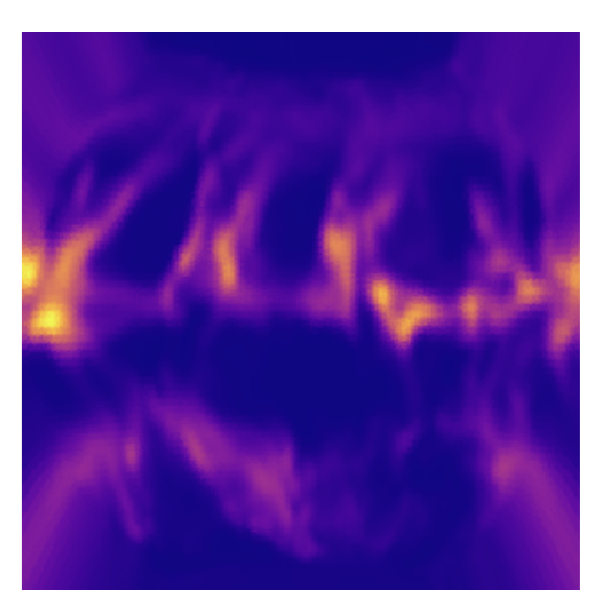
\includegraphics[width=0.9\linewidth]{figures/chapter-8/prect_wag.png}
%         \caption{Precipitation raster data as Wagner VII projected}
%         \label{fig:wag_prect_raster}
%     \end{minipage}\hfill
% \end{figure}

\subsection{Results and Observations}
\begin{table}[ht]
    \caption{Summary of Planar(Azimuthal) Projection Model Performance}
    \label{planner_results_table}
    \renewcommand{\arraystretch}{1.2} % Adjusts the row height
    \begin{tabular}{|l|c|c|c|c|c|}
        \hline
        \rowcolor[gray]{0.9}
        \textbf{\emph{Projection}}   & \textbf{\emph{\# Epochs}} & \textbf{\emph{MAE}} & \textbf{\emph{Validation MAE}} & \textbf{\emph{Loss}} & \textbf{\emph{Validation Loss}} \\ \hline
        Azimuthal Equidistant        & 20                        & 0.621               & 0.634                          & 0.697                & 0.725                           \\ \hline
        Wagner VII                   & 20                        & 0.609               & 0.627                          & 0.677                & 0.710                           \\ \hline
        Lambert Azimuthal Equal Area & 20                        & 0.676               & 0.680                          & 0.798                & 0.803                           \\ \hline
        Airy                         & 20                        & 0.768               & 0.787                          & 0.978                & 0.994                           \\ \hline
    \end{tabular}
\end{table}
